% !TEX TS-program = pdflatex
% !TEX encoding = UTF-8 Unicode

% This is a simple template for a LaTeX document using the "article" class.
% See "book", "report", "letter" for other types of document.

\documentclass[14pt]{article} % use larger type; default would be 10pt

\usepackage[utf8]{inputenc} % set input encoding (not needed with XeLaTeX)

%%% Examples of Article customizations
% These packages are optional, depending whether you want the features they provide.
% See the LaTeX Companion or other references for full information.

%%% PAGE DIMENSIONS
\usepackage{geometry} % to change the page dimensions
\geometry{a4paper,left = 40mm,top=35mm,right = 30mm,bottom=15mm,} % or letterpaper (US) or a5paper or....
% \geometry{margin=2in} % for example, change the margins to 2 inches all round
% \geometry{landscape} % set up the page for landscape
%   read geometry.pdf for detailed page layout information

\usepackage{graphicx} % support the \includegraphics command and options
\usepackage{mdframed}

% \usepackage[parfill]{parskip} % Activate to begin paragraphs with an empty line rather than an indent
\usepackage{float}
\usepackage{titling}
\usepackage{caption}
\usepackage{subcaption}
\setlength{\parindent}{4em}
%%% PACKAGES
\usepackage{booktabs} % for much better looking tables
\usepackage{array} % for better arrays (eg matrices) in maths
\usepackage{paralist} % very flexible & customisable lists (eg. enumerate/itemize, etc.)
\usepackage{verbatim} % adds environment for commenting out blocks of text & for better verbatim
%\usepackage{subfig} % make it possible to include more than one captioned figure/table in a single float
% These packages are all incorporated in the memoir class to one degree or another...

%%% HEADERS & FOOTERS
\usepackage{fancyhdr} % This should be set AFTER setting up the page geometry
\pagestyle{fancy} % options: empty , plain , fancy
\renewcommand{\headrulewidth}{1pt} % customise the layout...
\lhead{}\chead{}\rhead{Project Report | DRDO}
\lfoot{}\cfoot{}\rfoot{\thepage}
\topmargin = -23pt
\headsep = 10pt
\renewcommand{\footrulewidth}{1pt}

%%% SECTION TITLE APPEARANCE
\usepackage{sectsty}
\allsectionsfont{\sffamily\mdseries\upshape} % (See the fntguide.pdf for font help)
% (This matches ConTeXt defaults)

%%% ToC(table of contents) APPEARANCE
\usepackage[nottoc,notlof,notlot]{tocbibind} % Put the bibliography in the ToC
\usepackage[titles,subfigure]{tocloft} % Alter the style of the Table of Contents
\usepackage{amsmath}
\usepackage{lmodern}
\usepackage{tcolorbox}
\usepackage{indentfirst}
\usepackage{changepage}
\renewcommand{\cftsecfont}{\rmfamily\mdseries\upshape}
\renewcommand{\cftsecpagefont}{\rmfamily\mdseries\upshape} % No bold!

%%% END Article customizations

%%% The "real" document content comes below...

%\date{} % Activate to display a given date or no date (if empty),
         % otherwise the current date is printed 
\date{}


\begin{document}

 \tableofcontents
\listoffigures

 %chapter 1
\title{\huge {CHAPTER 1}}
\maketitle
\section{\huge{INTRODUCTION}}


\subsection{INTRODUCTION}
         Radar systems are generally used in determining properties, most commonly distance from a reference point of solid objects using single antennas or large antenna arrays. These antennas transmit and receive electromagnetic signals, which can be processed to obtain various relevant data. By using only one antenna and moving it along a linear axis to record an area of static objects, one can mimic a larger array of antennas to collect high-resolution data: this setup is known as a synthetic aperture radar system. The data collected from this type of radar configuration, after processing, is well-known for its detail and map-like quality and can be used to render a two-dimensional and three-dimensional representation of scanned area.
         
 \begin{figure}[t]
 \centering
 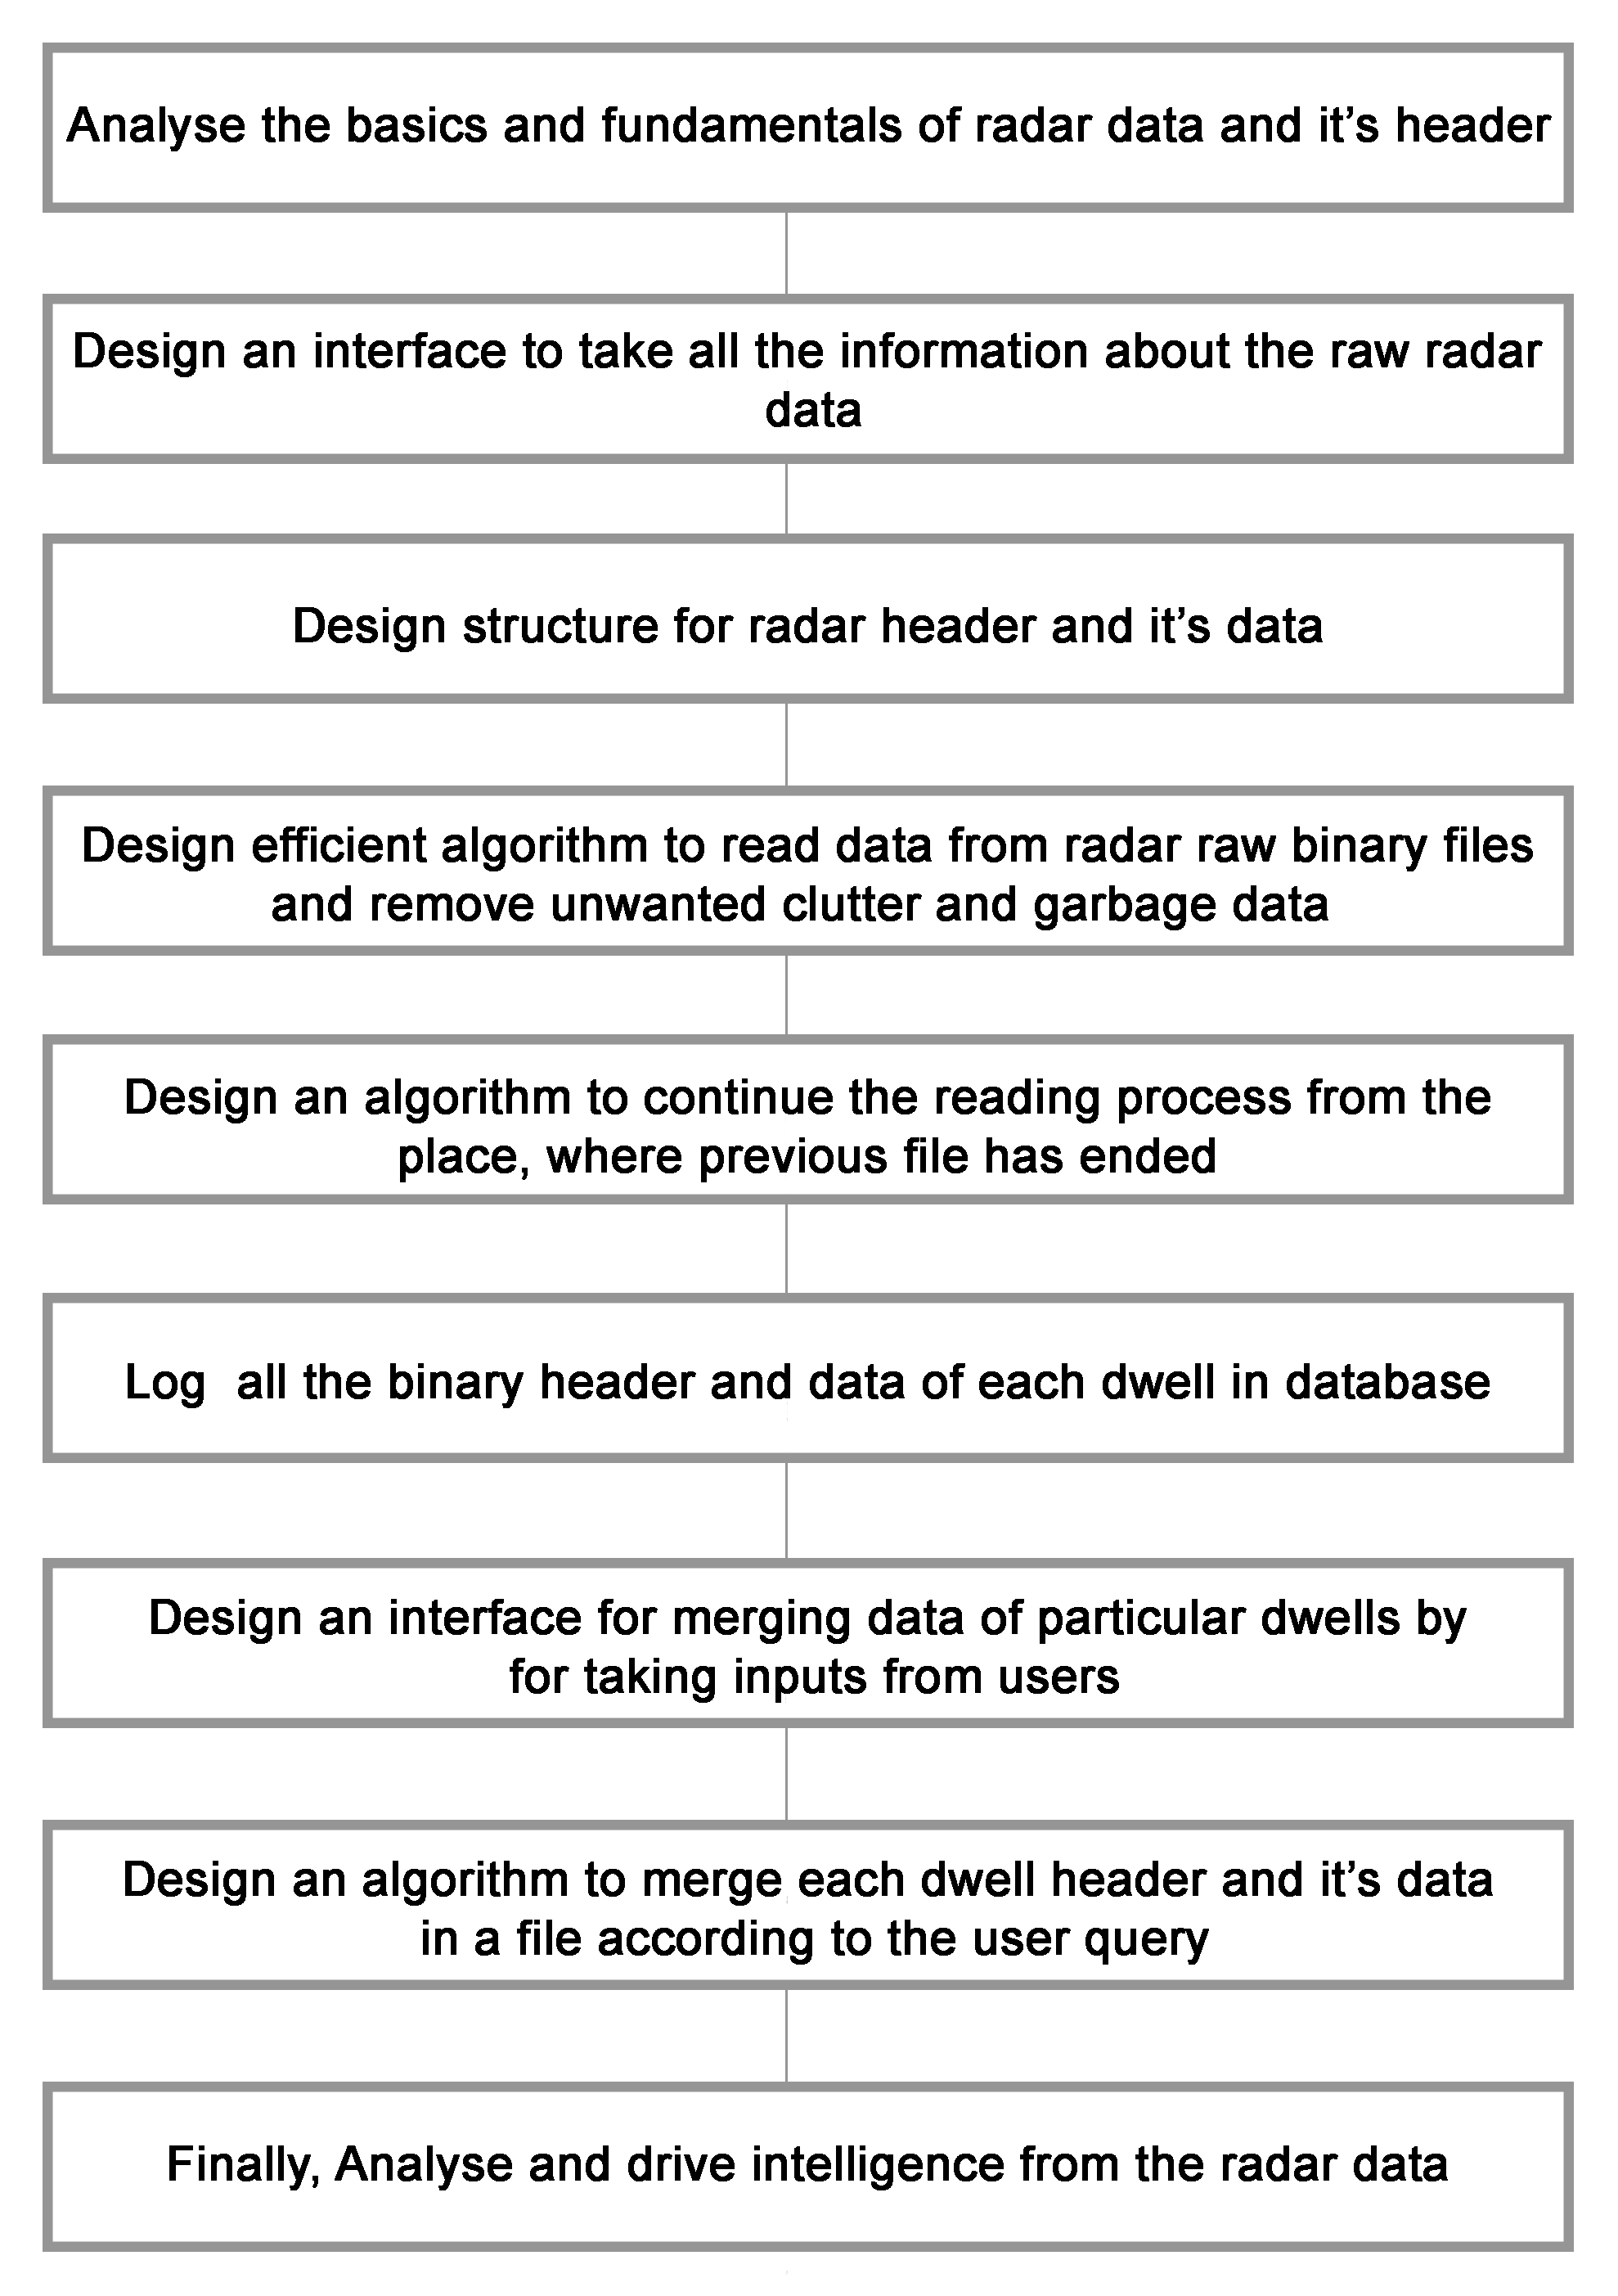
\includegraphics[width=0.8\linewidth]{steps.png}
  \caption{Steps involved.}
  \label{fig:figure 1}
\end{figure}
\end{document}